% \documentclass[handout]{beamer}
\documentclass[aspectratio=169]{beamer}

\mode<presentation>
{
  \usetheme{default}
  % \usefonttheme[onlymath]{serif}
  % \usetheme{Singapore}
  % \usetheme{Warsaw}
  % \usetheme{Malmoe}
  % \useinnertheme{circles}
  % \useoutertheme{infolines}
  % \useinnertheme{rounded}

  \setbeamercovered{transparent=20}
}

\usepackage{amssymb}
\usepackage[english]{babel}
\usepackage[latin1]{inputenc}
\usepackage{alltt,listings,multirow,ulem,siunitx}
\usepackage[absolute,overlay]{textpos}
\TPGrid{1}{1}
\usepackage{pdfpages}
\usepackage{ulem}
\usepackage{multimedia}
\usepackage{multicol}
\usepackage{transparent}
\newcommand\hmmax{0}
\newcommand\bmmax{0}
\usepackage{bm}
\usepackage{comment}
\usepackage{subcaption}

% font definitions, try \usepackage{ae} instead of the following
% three lines if you don't like this look
\usepackage{mathptmx}
\usepackage[scaled=.90]{helvet}
% \usepackage{courier}
\usepackage[T1]{fontenc}
\usepackage{tikz}
\usetikzlibrary{decorations.pathreplacing}
\usetikzlibrary{shadows,arrows,shapes.misc,shapes.arrows,shapes.multipart,arrows,decorations.pathmorphing,backgrounds,positioning,fit,petri,calc,shadows,chains,matrix,mindmap}

\newcommand\vvec{\bm v}
\newcommand\bvec{\bm b}
\newcommand\bxk{\bvec_0 \times \kappa_0 \cdot \nabla}
\newcommand\delp{\nabla_\perp}

% \usepackage{pgfpages}
% \pgfpagesuselayout{4 on 1}[a4paper,landscape,border shrink=5mm]

\usepackage{JedMacros}

\newcommand{\timeR}{t_{\mathrm{R}}}
\newcommand{\timeW}{t_{\mathrm{W}}}
\newcommand{\mglevel}{\ensuremath{\ell}}
\newcommand{\mglevelcp}{\ensuremath{\mglevel_{\mathrm{cp}}}}
\newcommand{\mglevelcoarse}{\ensuremath{\mglevel_{\mathrm{coarse}}}}
\newcommand{\mglevelfine}{\ensuremath{\mglevel_{\mathrm{fine}}}}

%solution and residual
\newcommand{\vx}{\ensuremath{x}}
\newcommand{\vc}{\ensuremath{\hat{x}}}
\newcommand{\vr}{\ensuremath{r}}
\newcommand{\vb}{\ensuremath{b}}

%operators
\newcommand{\vA}{\ensuremath{A}}
\newcommand{\vP}{\ensuremath{I_H^h}}
\newcommand{\vS}{\ensuremath{S}}
\newcommand{\vR}{\ensuremath{I_h^H}}
\newcommand{\vI}{\ensuremath{\hat I_h^H}}
\newcommand{\vV}{\ensuremath{\mathbf{V}}}
\newcommand{\vF}{\ensuremath{F}}
\newcommand{\vtau}{\ensuremath{\mathbf{\tau}}}


\title{Physically-based Prediction, Inference, and Design}
\author{Jed Brown}

% - Use the \inst command only if there are several affiliations.
% - Keep it simple, no one is interested in your street address.
% \institute
% {
%   Mathematics and Computer Science Division \\ Argonne National Laboratory
% }

\date{Applied Math Graduate Seminar, 2018-02-28}
%    - **SW**: miniapps: Nekbone, Laghos, NekCEM Ceedling, HPGMG-FE, HOLMES; CEED distribution/Spack; HO visualization ALPINE, VTK-m, iLight… HO data format; GSLIB; MPICH collaboration; high-order meshes, PUMI; solvers: Strumpack, PETSC, matrix-free; zfp;  

% This is only inserted into the PDF information catalog. Can be left
% out.
\subject{Talks}


% If you have a file called "university-logo-filename.xxx", where xxx
% is a graphic format that can be processed by latex or pdflatex,
% resp., then you can add a logo as follows:

% \pgfdeclareimage[height=0.5cm]{university-logo}{university-logo-filename}
% \logo{\pgfuseimage{university-logo}}



% Delete this, if you do not want the table of contents to pop up at
% the beginning of each subsection:
% \AtBeginSubsection[]
% {
% \begin{frame}<beamer>
%   \frametitle{Outline}
%   \tableofcontents[currentsection,currentsubsection]
% \end{frame}
% }

\AtBeginSection[]
{
  \begin{frame}<beamer>
    \frametitle{Outline}
    \tableofcontents[currentsection]
  \end{frame}
}

% If you wish to uncover everything in a step-wise fashion, uncomment
% the following command:

% \beamerdefaultoverlayspecification{<+->}

\begin{document}
\lstset{language=C}
\normalem

\setbeamercolor{background canvas}{bg=}

\begin{frame}
  \begin{center}
    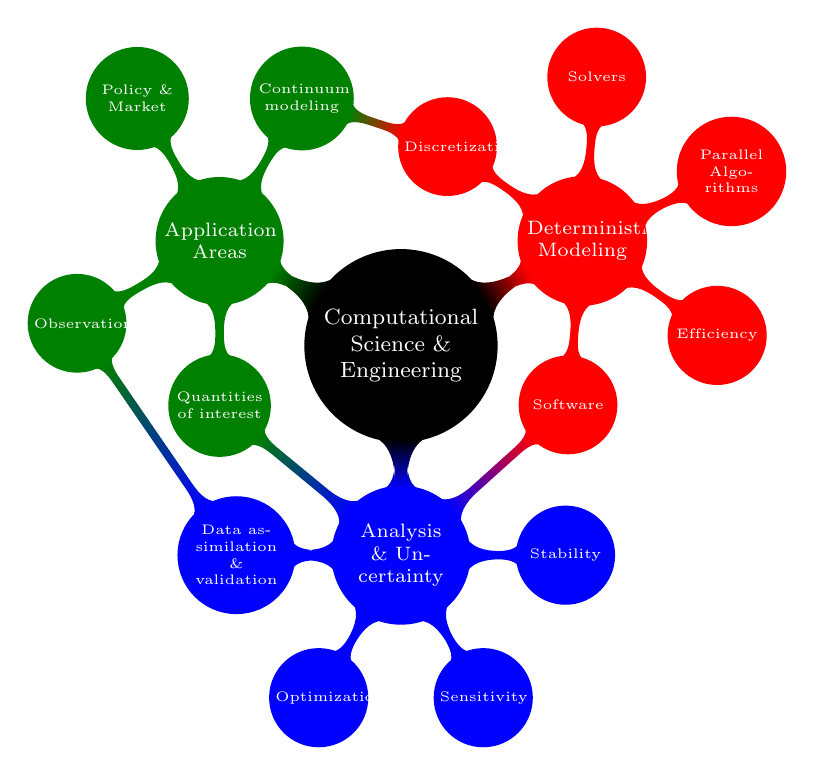
\begin{tikzpicture}
      [scale=0.95,small mindmap,concept color=black,text=white,
      %level 1 concept/.append style={level distance=120,sibling angle=30},
      extra concept/.append style={color=blue!50,text=black}]

      \node [concept] {Computational Science \& Engineering}
      child [concept color=green!50!black,grow=150] {
        node [concept] {Application \\ Areas}[counterclockwise from=60]
        child {node [concept] (cont) {Continuum modeling}}
        child {node [concept] (policy) {Policy \& Market}}
        child[grow=-150] {node [concept] (obs) {Observation}}
        child[grow=-90] {node [concept] (qoi) {Quantities of interest}}
      }
      child [concept color=red,text=white,grow=30] {
        node [concept] {Deterministic Modeling}[clockwise from=145,sibling angle=25]
        child {node [concept] (disc) {Discretization}}
        child {node [concept] (solver) {Solvers}}
        child {node [concept] (alg) {Parallel Algorithms}}
        child {node [concept] (eff) {Efficiency}}
        child {node [concept] (software) {Software}}
      }
      child [concept color=blue,text=white,grow=-90] {
        node[concept] (analysis) {Analysis \& Uncertainty}[clockwise from=0]
        child {node [concept] (stab) {Stability}}
        child {node [concept] (sens) {Sensitivity}}
        child {node [concept] (opt) {Optimization}}
        child {node [concept] (assim) {Data assimilation \\ \& validation}}
      }
      ;
      \begin{pgfonlayer}{background}
        \path (analysis) to[circle connection bar switch color=from (blue) to (red)] (software);
        \path (cont) to[circle connection bar switch color=from (green!50!black) to (red)] (disc);
        \path (qoi) to[circle connection bar switch color=from (green!50!black) to (blue)] (analysis);
        \path (obs) to[circle connection bar switch color=from (green!50!black) to (blue)] (assim);
      \end{pgfonlayer}
    \end{tikzpicture}
  \end{center}
\end{frame}


\begin{frame}{Computational geodynamics}
  \begin{center}
    \includegraphics[width=.8\textwidth]{figures/davemay/MayGeodynamicsTimeline.png}
  \end{center}
  \vspace{-1ex}
  {\scriptsize Figure adapted from Taras Gerya}
\end{frame}

\begin{frame}{Regional scale geodynamic processes}
  \begin{center}
    \includegraphics[width=.65\textwidth]{figures/davemay/WPRegionalGeodynamicsProcesses.png}
  \end{center}
  \begin{columns}
    \begin{column}{0.5\textwidth}
      \begin{itemize}
      \item Buoyancy and topography drive flow
      \item Large variation in length scales
      \item Small scales influence large scales
      \end{itemize}
    \end{column}
    \begin{column}{0.5\textwidth}
      \begin{itemize}
      \item Complex rheology (research)
      \item Material failure (faults)
      \item Post-failure deformation
      \item Thermomechanically coupled
      \end{itemize}
    \end{column}
  \end{columns}
\end{frame}
\begin{frame}{Continental rifting}
  %\movie[width=\textwidth,height=0.66\textwidth,autostart,poster,showcontrols=false,loop]{Oblique Rifting Video}{dstrong2_truc.mov}
  \begin{center}
    \movie[width=.8\textwidth,height=0.66\textwidth,autostart,poster,showcontrols=false,loop]{Rifting Video}{LaetiSC14Rifting.mp4}
  \end{center}
\end{frame}

\begin{frame}{Continuum modeling}
  %Solve for velocity $\bm u$, pressure $p$, temperature $T$, materials
  %$\rho_i$
  \begin{itemize}
  \item Something we trust: \textbf{Conservation}
    \begin{align*}
      -\nabla\cdot \big[ \eta D \bm u - p \bm I \big] &= \rho \bm g & \text{momentum} \\
      \nabla \cdot \rho \bm u &= 0 & \text{mass} \\
      \frac{\partial T}{\partial t} + \nabla\cdot (\bm u T - \kappa \nabla T) &= Q & \text{energy} \\
      \frac{\partial \Phi_i}{\partial t} + \nabla\cdot (\bm u \Phi_i) &= 0, \quad \sum_i\Phi_i=1 & \text{composition}
    \end{align*}
    \begin{itemize}
    \item Non-Newtonian Stokes, high-contrast coefficients $10^{10}$
    \item Boussinesq approximation, high Rayleigh number, zero Reynolds
    \end{itemize}
  \item Something we don't: \textbf{Constitutive models}
    \begin{itemize}
    \item $\eta(D\bm u,p,T,\Phi_i)$ shear viscosity---viscoplastic, non-smooth
    \item $\rho(p,T,\Phi_i)$ density
    \item $\kappa(T, \Phi_i)$ thermal diffusivity
    \item Initial and boundary conditions, geometry
    \end{itemize}
  \end{itemize}
\end{frame}

\begin{frame}{Materials: Molecular dynamics to continuum}
  \begin{itemize}
  \item Molecular Dynamics
    \begin{itemize}
    \item Possible scales: a few nanometers, nanosecond to microsecond
    \item Deterministic input: density, temperature, composition/purity
    \item Stochastic: initialize atom locations and momentum
    \item Simulate: evolve for millions of time steps using force models
    \item Integrate: heat flux, other macroscopic quantities
    \end{itemize}
  \item Continuum models for larger space/time scales
    \begin{itemize}
    \item We trust: conservation of mass, momentum, energy; entropy
    \item ML problem: derive effective models using MD simulations
    \item Regression, derivation of new macroscopic variables
    \end{itemize}
  \item Interdisciplinary Research Theme: 2-4 month proof of concept
    \begin{itemize}
    \item Initial target: thermoelectric materials: heat flux $\Longleftrightarrow$ electric current
    \item Future applications: nanotube composites, photovoltaics, battery technologies
    \item With Sanghamitra Neogi (Aerospace)
    \end{itemize}
  \end{itemize}
\end{frame}

\begin{frame}{PETSc: Portable Extensible Toolkit for Scientific Computing}
  \begin{itemize}
  \item Optimization: $\argmin_u f(u), g(u) = 0, h(u) \ge 0$
  \item Time integration: $f(t, u, \dot u) = g(t, u)$
    \begin{itemize}
    \item Implicit, explicit, IMEX, with adjoints and events
    \end{itemize}
  \item Nonlinear solvers: $F(u) = 0$
  \item Eigensolvers (SLEPc): $A u = \lambda u$
  \item Linear solvers: $A u = b$
  \item Discretization tools: structured, unstructured
  \item Pervasive support for multilevel methods
  \item Used by many applications and libraries, research and industry
  \item Prizes: SIAM/ACM CS\&E, R\&D 100, 5 Gordon Bell
  \end{itemize}
\end{frame}

\input{slides/PETSc/Composition.tex}

\includepdf[pages=2-3]{figures/ceed/1am/fy17-review.pdf}
\includepdf[pages=7]{figures/ceed/1am/CEED1AM-FuturePlans.pdf} % High Order Software Ecosystem
\includepdf[pages=7]{figures/ceed/1am/fy17-review.pdf} % CEED Software Products
\includepdf[pages=46]{/home/jed/ceed/ceed/talks/CEED-ECP-FY17-Review-Aug-2017.pdf} % Applicable to variety of physics

\begin{frame}{Active Learning/Experimental Design}
  \begin{columns}
    \begin{column}{0.4\textwidth}
      \includegraphics[width=\textwidth]{figures/al-amr/shockbubble_level_4a.pdf} \\
      \includegraphics[width=\textwidth]{figures/al-amr/shockbubble_level_5a.pdf} \\
      \includegraphics[width=\textwidth]{figures/al-amr/shockbubble_level_6a.pdf}
    \end{column}
    \begin{column}{0.6\textwidth}
      \includegraphics[width=\textwidth]{figures/al-amr/rmse-RGMA-and-RG.pdf}
    \end{column}
  \end{columns}
\end{frame}

\begin{frame}{Outlook}
  \begin{itemize}
  \item Application areas
    \begin{itemize}
    \item Geodynamics and Geophysics
    \item Materials Science (all scales)
    \item Aerospace Engineering and CFD
    \item Energy Sciences: Fission Reactors, Wind, Geothermal 
    \end{itemize}
  \item Funding sources
  \begin{itemize}
  \item DOE ASCR
  \item DOE ECP
  \item DOE BER SciDAC
  \item NSF SI2
  \end{itemize}
  \end{itemize}
\end{frame}

\end{document}
